% Currículo de João Gabriel Salvador Paiva — perfil generalista de desenvolvimento de software
% Layout de coluna única, texto 100% selecionável, sem tabelas nem caixas de texto (ATS-friendly).
\documentclass[10.5pt,a4paper]{article}

\usepackage[T1]{fontenc}
\usepackage[utf8]{inputenc}
\usepackage{lmodern}
\usepackage[margin=1.5cm,top=1.2cm,bottom=1.2cm]{geometry}
\usepackage{graphicx}
\usepackage{enumitem}
\usepackage{titlesec}
\usepackage{xcolor}
\usepackage[hidelinks]{hyperref}
\usepackage{microtype}
\usepackage{needspace}

\definecolor{azul}{HTML}{14375A}

\hypersetup{
  pdftitle={Joao Gabriel Salvador Paiva - Desenvolvedor de Software},
  pdfauthor={Joao Gabriel Salvador Paiva},
  pdfsubject={Curriculo - Desenvolvedor de Software},
  pdfkeywords={Python, Dart, Django, FastAPI, APIs REST, microsservicos, Flutter, PostgreSQL, Redis,
  RabbitMQ, Docker, AWS, GitHub Actions, CI/CD, PyTest, Clean Code, SOLID, Scrum, LLMs}
}

\pagestyle{empty}
\setlength{\parindent}{0pt}
\setlength{\emergencystretch}{2em}
\setlist[itemize]{leftmargin=3.6mm,itemsep=1pt,topsep=2pt,parsep=0pt,label=\textbullet}

\titleformat{\section}{\bfseries\large\color{azul}}{}{0em}{}[\vspace{-1.2ex}\rule{\linewidth}{0.6pt}]
\titlespacing{\section}{0pt}{2.2ex}{1.2ex}

\newcommand{\cargo}[4]{%
  \Needspace*{5\baselineskip}%
  \textbf{#1} \textnormal{---} #2 \hfill \textnormal{#3}\\
  \textit{\small #4}\vspace{0.4ex}
}

\begin{document}

%% ---------- Cabeçalho ----------
\begin{minipage}[c]{0.78\textwidth}
\raggedright
{\LARGE\bfseries\color{azul} João Gabriel Salvador Paiva}\\[0.6ex]
{\large Desenvolvedor de Software}\\[0.9ex]
\small
Campina Grande – PB, Brasil (disponível para trabalho remoto)\\
\href{mailto:joaogabrielsalvadorpaiva@gmail.com}{joaogabrielsalvadorpaiva@gmail.com} $\cdot$ +55 (83) 98863-6734\\
\href{https://github.com/Ilusinusmate}{github.com/Ilusinusmate} $\cdot$
\href{https://www.linkedin.com/in/joao-gabriel-salvador-paiva-805283286}{linkedin.com/in/joao-gabriel-salvador-paiva} $\cdot$
\href{https://ilusinusmate.github.io/Ilusinusmate/}{ilusinusmate.github.io/Ilusinusmate}
\end{minipage}\hfill
\begin{minipage}[c]{0.2\textwidth}
\raggedleft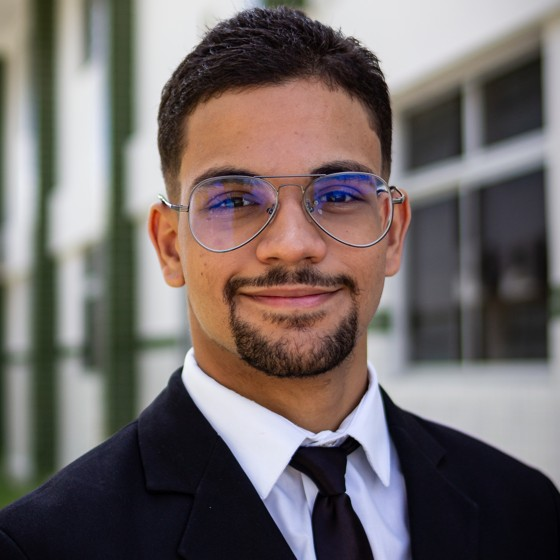
\includegraphics[width=2.7cm]{foto.jpg}
\end{minipage}

%% ---------- Resumo ----------
\section*{Resumo}
Desenvolvedor de software com experiência em \textbf{backend Python} e desenvolvimento
\textbf{mobile com Flutter/Dart}, construindo \textbf{APIs REST}, microsserviços e aplicações em
produção. Na Logon, sou responsável pelo app \textbf{Central da Escola}, com mais de
\textbf{50 mil usuários ativos}, e por serviços de apoio em Python/FastAPI, além de conduzir
testes, CI/CD e publicação nas lojas Android e iOS. Também construí um SaaS de ERP, PDV e
e-commerce com Django/Python e PostgreSQL, e atuo em pesquisa sobre IA, LLMs e Engenharia de
Software. Graduando em Ciência da Computação na UFCG e residente em TIC no VIRTUS-CC/UFCG.

%% ---------- Competências ----------
\section*{Competências técnicas}
\textbf{Linguagens:} Python, Dart, JavaScript, TypeScript, SQL, C\\
\textbf{Backend:} Django, Django REST Framework, FastAPI, APIs REST, microsserviços, autenticação,
integrações entre sistemas\\
\textbf{Mobile:} Flutter, Dart, Android, iOS, publicação nas lojas, BLoC, WebSocket, componentização\\
\textbf{Dados:} PostgreSQL, bancos NoSQL, Redis, MinIO, modelagem de dados\\
\textbf{Infra e DevOps:} RabbitMQ, Docker, AWS (S3, CloudFront), Railway, Render, Nginx, Linux,
GitHub Actions, CI/CD, OpenTelemetry, Grafana, logging\\
\textbf{Qualidade:} PyTest, mocks, testes automatizados, code review\\
\textbf{Engenharia:} Clean Code, SOLID, DRY, DDD, design patterns, documentação técnica,
Scrum/Kanban, sistemas distribuídos

%% ---------- Experiência ----------
\section*{Experiência profissional}

\cargo{Logon Informática}{Mobile \& Backend Developer}{jan/2025 -- atual}{Software house de
sistemas de gestão para educação, administração pública e outros setores}
\begin{itemize}
  \item Desenvolvo microsserviços em \textbf{Python/FastAPI}, APIs REST, comunicação assíncrona com
        \textbf{RabbitMQ} e armazenamento de objetos com \textbf{MinIO} para o app Central da Escola.
  \item Sou o único desenvolvedor do aplicativo desde a \textbf{versão 3}, em
        \textbf{Flutter/Dart}, com mais de \textbf{50 mil usuários ativos} em Android e iOS.
  \item Lidero o setor mobile e conduzo desenvolvimento, testes, \textbf{CI/CD}, publicação nas
        lojas, logging, documentação e mediação com times internos e sistemas de terceiros.
\end{itemize}

\cargo{Empório Sertanejo}{Desenvolvedor Full-stack --- líder técnico}{dez/2023 -- set/2025}{Franquia
de varejo; SaaS proprietário de ERP, PDV e e-commerce}
\begin{itemize}
  \item \textbf{Liderei 3 desenvolvedores} na construção de um SaaS que unificou
        \textbf{ERP, PDV e e-commerce}, usando \textbf{Django/Python}, \textbf{PostgreSQL} e
        \textbf{Docker}.
  \item Implementei testes automatizados com PyTest e mocks, CI/CD com GitHub Actions e
        observabilidade com OpenTelemetry e Grafana.
  \item Conduzi levantamento de requisitos e negociação com o cliente, entregando programa de
        pontos, cupons, notificações e vendas online.
\end{itemize}

\cargo{VIRTUS-CC / Softex (UFCG)}{Residente em TIC --- pesquisador do grupo ISE}{nov/2025 --
atual}{Programa de residência em software de 1 ano: 240h de capacitação + imersão prática}
\begin{itemize}
  \item Aprovado em \textbf{1º lugar} no processo seletivo (96/100 na prova de títulos e 100/100 na
        entrevista).
  \item Formação em Engenharia de Software, metodologias ágeis, IoT, machine learning e design
        thinking, com projetos em squad multidisciplinar.
  \item Pesquiso LLMs aplicados à Engenharia de Software no grupo \textbf{Intelligent Software
        Engineering}, com artigo aceito no \textbf{XP 2026} (Springer LNBIP).
\end{itemize}

\cargo{Animalesko}{Desenvolvedor Backend (voluntário)}{abr/2024 -- set/2024}{Startup social de apoio
a animais de rua}
\begin{itemize}
  \item Projetei a arquitetura backend multiplataforma do aplicativo, priorizando baixo consumo de
        recursos, e documentei as decisões técnicas.
\end{itemize}

\cargo{IFPB (CNPq / LAPLIN)}{Pesquisador bolsista e professor de Python}{2023 -- 2024}{Laboratório de
Análise e Processamento de Linguagem Natural}
\begin{itemize}
  \item Fui bolsista de pesquisa, com liderança do grupo discente em dois projetos, e ministrei
        aulas de \textbf{Python} para cerca de 60 alunos.
  \item Conduzi experimento comparando o aprendizado de programação com e sem apoio de IA, com
        publicações em eventos nacionais.
\end{itemize}

%% ---------- Projetos ----------
\section*{Projetos}
\begin{itemize}
  \item \textbf{pdfa-parser} --- biblioteca Python open source publicada no PyPI para conversão de
        PDFs ao padrão PDF/A e validação automática com GhostScript e VeraPDF, com APIs síncrona e
        assíncrona, CLI e execução em contêiner:
        \href{https://pypi.org/project/pdfa-parser}{pypi.org/project/pdfa-parser}
  \item \textbf{Contratexto} --- jogo web multiplayer em FastAPI com WebSocket e similaridade
        semântica, usando NLP e fila assíncrona:
        \href{https://contratexto.onrender.com}{contratexto.onrender.com}
  \item \textbf{Central da Escola} --- aplicativo escolar em Flutter com mais de
        \textbf{50 mil usuários ativos}, publicado em Android e iOS, com microsserviços próprios.
  \item \textbf{TodoApp} --- aplicativo Flutter com Clean Code, SOLID, componentização, context
        isolation e BLoC, executado em Android e Linux Desktop:
        \href{https://github.com/Ilusinusmate/todoApp}{github.com/Ilusinusmate/todoApp}
  \item \textbf{Corretor ONHB} --- aplicativo feito a pedido de professores do IFPB para correção
        automática de provas da Olimpíada Nacional em História do Brasil, em Flutter e Electron.
\end{itemize}

%% ---------- Formação ----------
\section*{Formação}
\textbf{Bacharelado em Ciência da Computação} --- Univ. Federal de Campina Grande (UFCG)
\hfill jan/2025 -- 2030\\
\textbf{Técnico Integrado} --- Instituto Federal da Paraíba (IFPB) \hfill mar/2022 -- dez/2024\\
\textbf{Formação complementar} --- Flutter Specialist e Python Backend Developer (DIO)

%% ---------- Publicações e prêmios ----------
\section*{Publicações e prêmios (seleção)}
\begin{itemize}
  \item \textbf{8 trabalhos científicos} publicados sobre IA, LLMs e Engenharia de Software,
        incluindo artigo no \textbf{XP 2026} (Springer LNBIP, 2º autor) e artigos no
        \textbf{WEI 2025} e \textbf{WICS 2024} (Sociedade Brasileira de Computação).
  \item \textbf{Melhor resumo expandido} da modalidade Iniciação Científica e Tecnológica --- TIC
        no \textbf{5º SIMPIF} (2023).
  \item \textbf{Campeão da Olimpíada Paraibana de Informática} (2023), \textbf{ouro} na categoria
        Avançado Júnior (2026) e finalista da Olimpíada Brasileira de Informática (2023).
\end{itemize}

\section*{Idiomas}
Português (nativo) $\cdot$ Inglês (avançado --- leitura, escrita e comunicação profissional)
$\cdot$ Libras (intermediário)

\end{document}
